\documentclass{beamer}
\usepackage[english,russian]{babel}
\usepackage[utf8]{inputenc}
\usepackage {xcolor}
\usetheme{Warsaw}
\usepackage{graphicx}  % Для вставки рисунков
\graphicspath{{Pictures/}{Pictures/}}  % папки с картинками
\setlength\fboxsep{3pt} % Отступ рамки \fbox{} от рисунка
\setlength\fboxrule{1pt}
\begin{document}

\title{\bf{Лондон}}  
\author{Каляев Тимур}
\institute{Московский государственный университет}
\date{Баку, 2019} 
\frame{\titlepage} 

\begin{frame}
\frametitle{Немного о столице}
Лондон --- столица и крупнейший город Соединённого Королевства Великобритании и Северной Ирландии.

Административно образует регион Англии, разделённый на 33 самоуправляемых территории. Население 
составляет 8,6 млн человек (2015 год) — это третий по величине город Европы.
\vskip 5 mm
\centering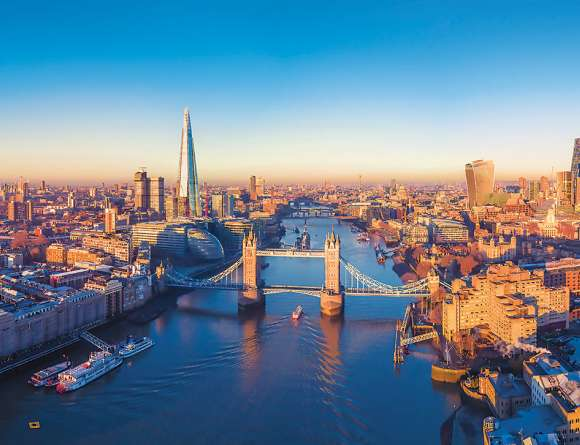
\includegraphics[width=0.5\linewidth]{london1.jpg}
\end{frame}

\begin{frame}
\frametitle{Немного экономики}
\begin{block}{Об экономике}
Лондон относится к глобальным городам высшего ранга и ведущим 
мировым финансовым центрам. Экономика его составляет пятую 
часть экономики страны. Лондон является одним из привлекательнейших городов для 
инвестиций, и в его юрисдикции зарегистировано наибольшее 
число международных торговых компаний и лиц со сверхкрупным 
чистым капиталом среди всех городов мира.
\end{block}
\centering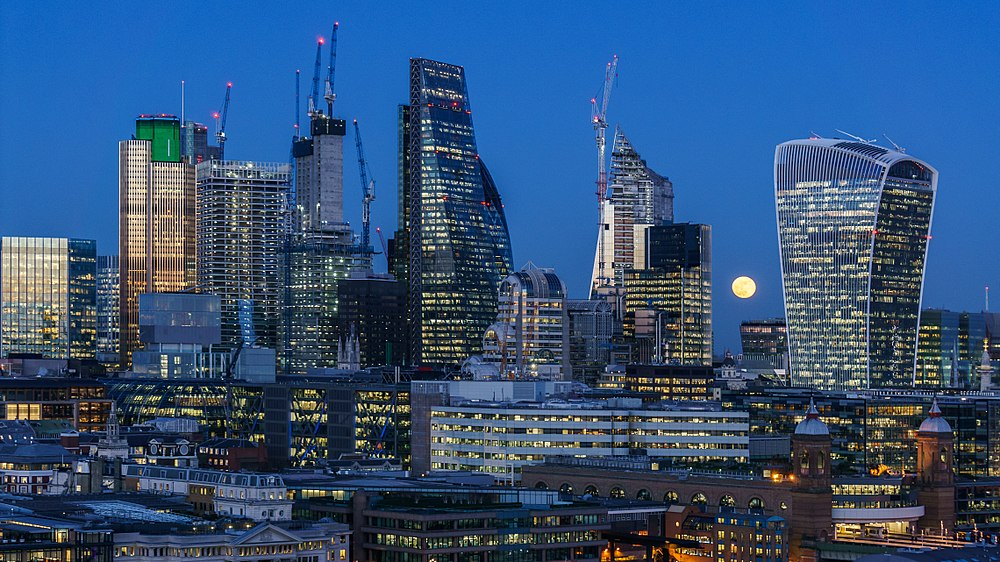
\includegraphics[width=0.5\linewidth]{london2.jpg} 
\end{frame}

\begin{frame}
\frametitle{Немного истории}
Основан римлянами вскоре после их вторжения в Британию 43 года н. э. 
Приблизительно с 100 года н. э. — столица римской Британии, 
с XI—XII столетий — Англии, с 1707 года — Великобритании, 
с XVI по XX век — Британской империи. 
С 1825 по 1925 год Лондон был крупнейшим городом мира.
\vskip 5 mm 
\centering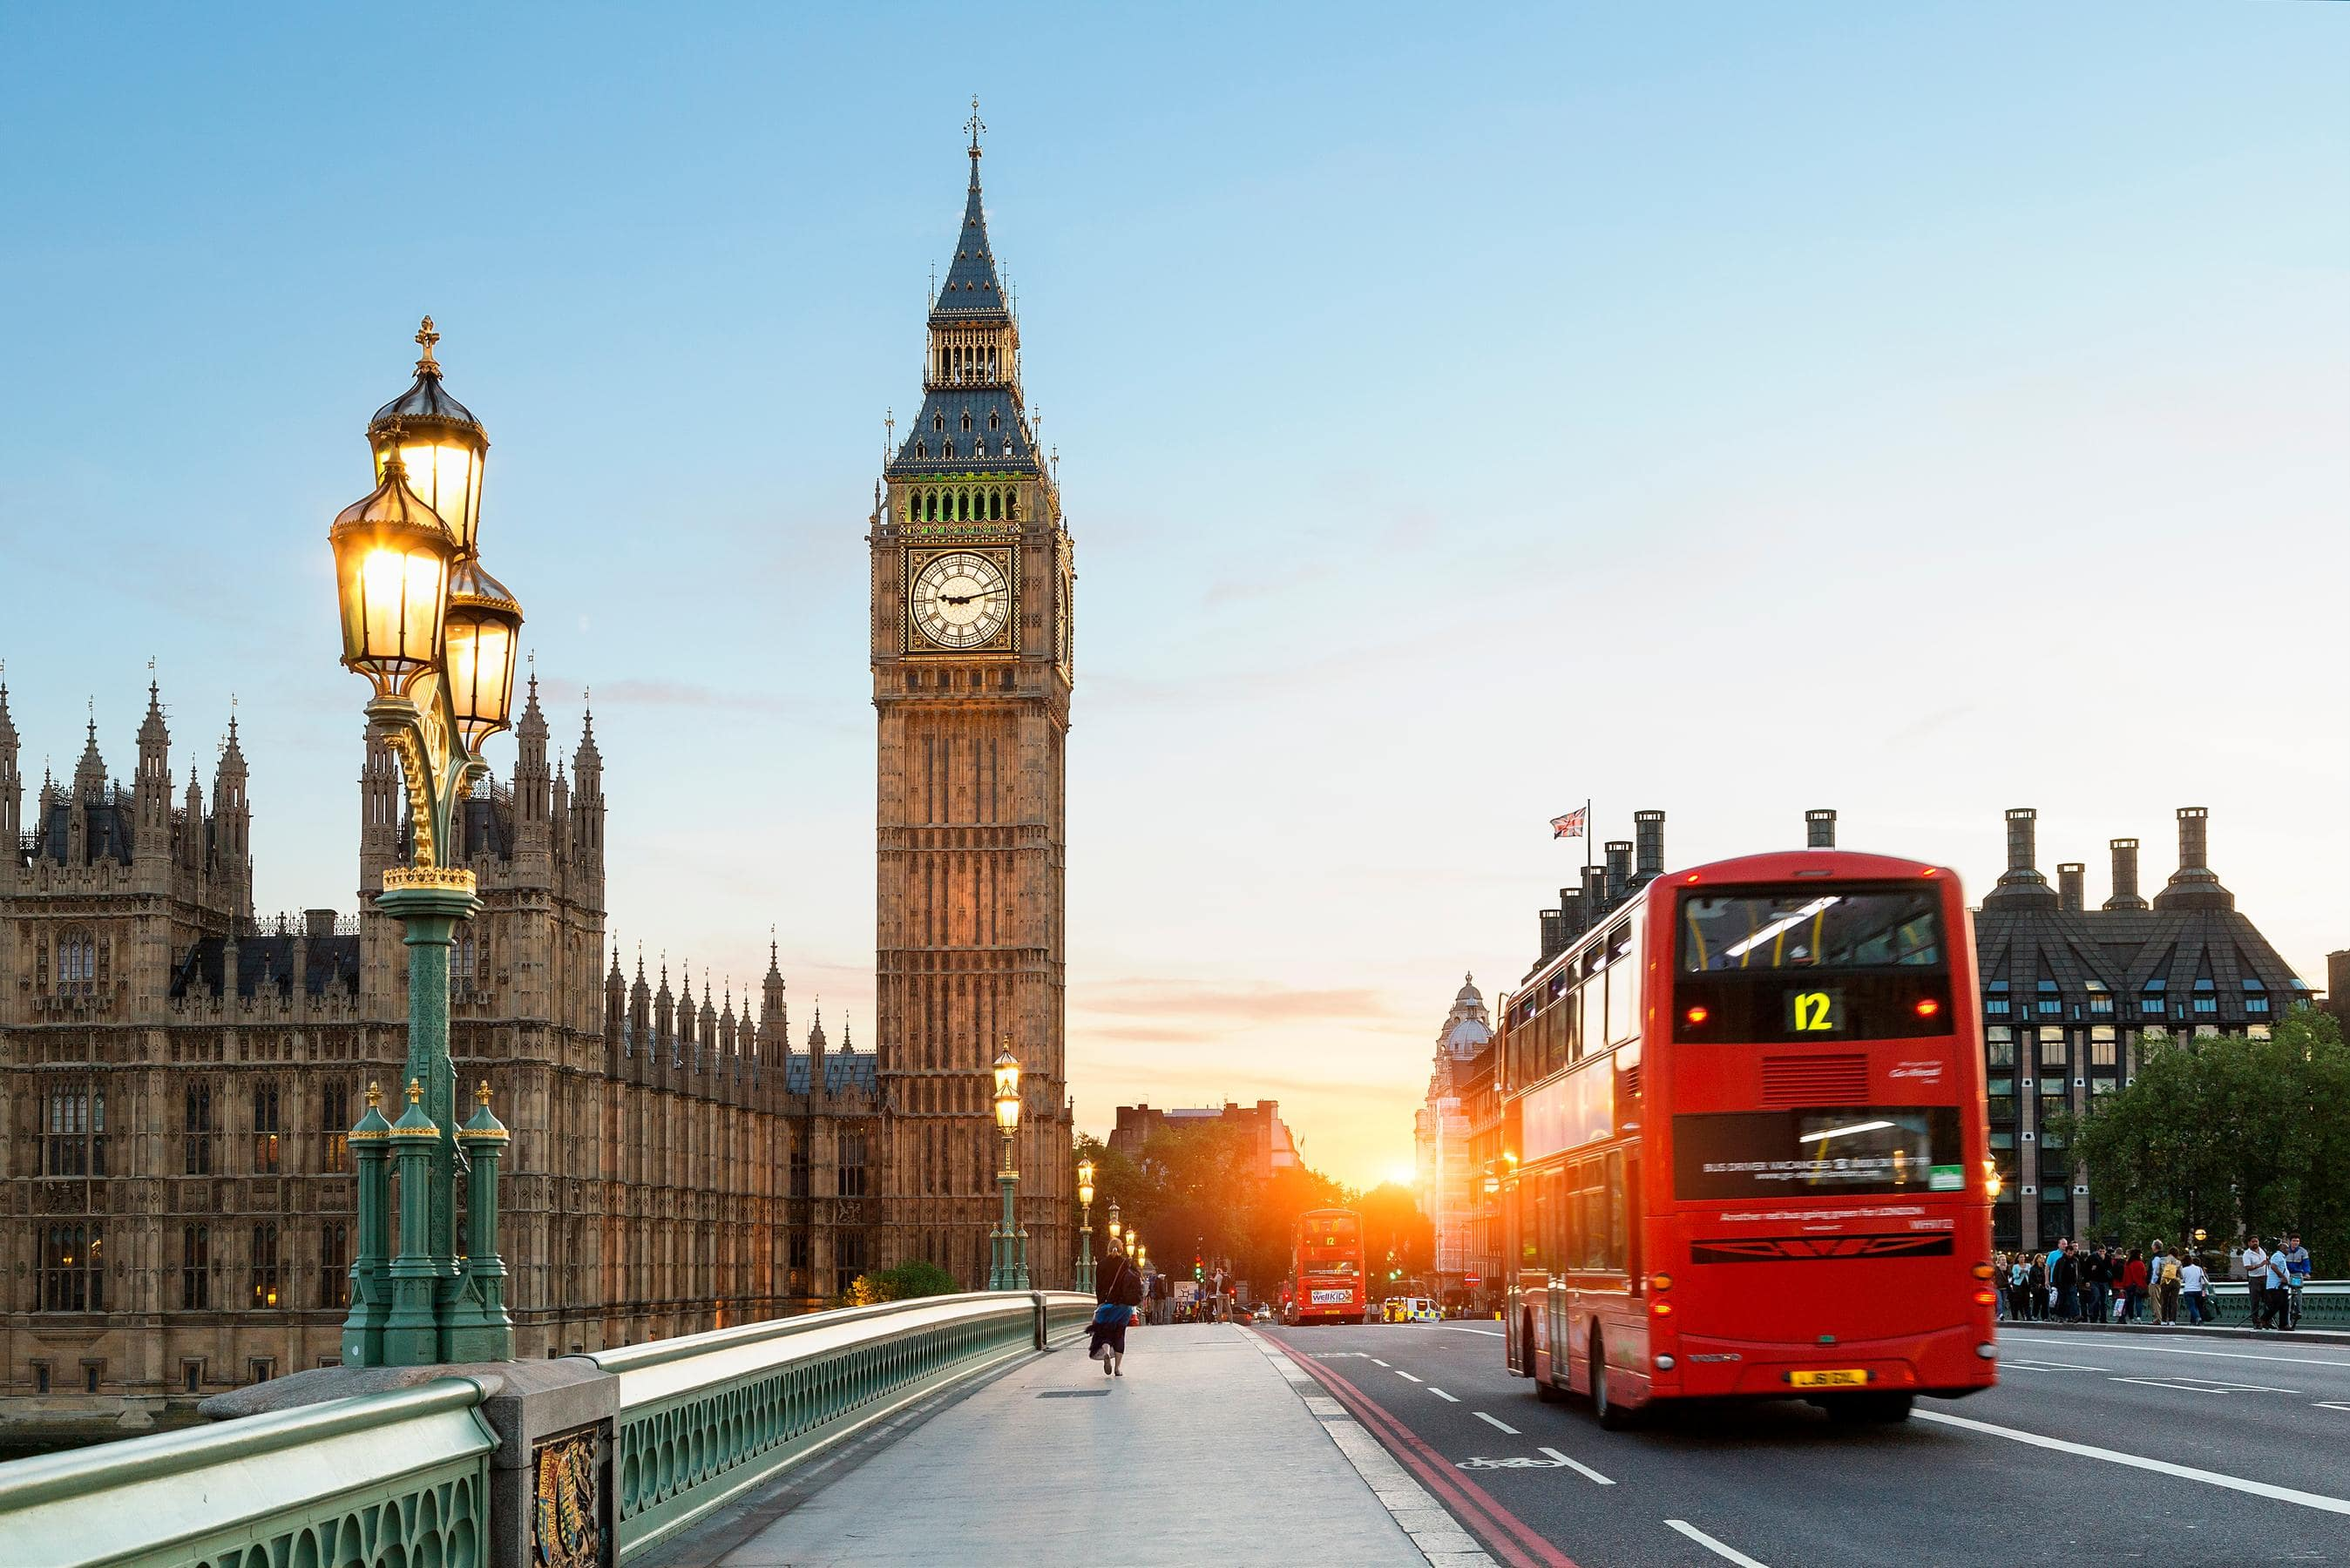
\includegraphics[width=0.5\linewidth]{london3.jpg}
\end{frame}

\begin{frame}
\frametitle{Немного о парках}
Восемь королевских парков, часть которых в прошлом были охотничьими угодьями королей, занимают площадь около 2000 га: Гайд-парк является 
крупнейшим в центре города, открытым для свободного посещения в 1826 году. Вместе с примыкающими к нему 
Кенсингтонскими садами образует зелёный массив общей площадью свыше 250 га, длиною свыше двух км и шириной свыше одного км. 
\vskip 5 mm 
\centering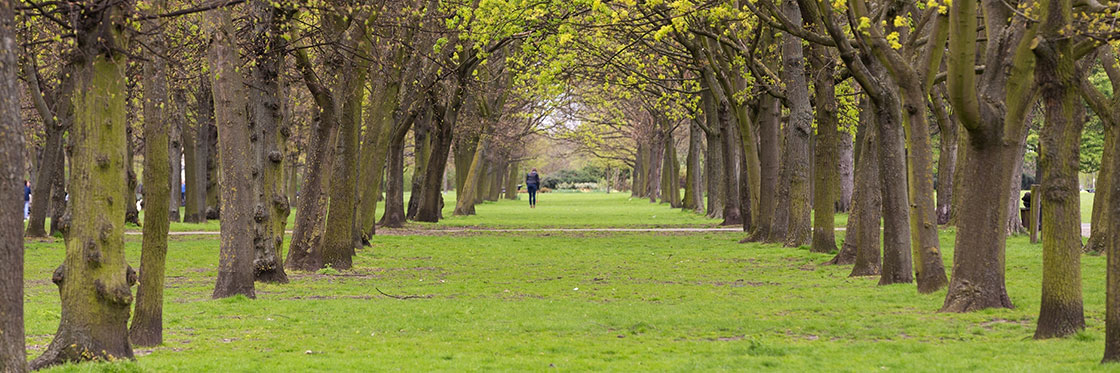
\includegraphics[width=1\linewidth]{park02.jpg}
\end{frame}

\begin{frame}
\frametitle{Немного о Букингемском двореце}
Букингемский дворец --- официальная лондонская резиденция 
британских монархов (в настоящее время --- королевы Елизаветы II). 
Расположен напротив улицы Мэлл и Грин-парка с беломраморным и 
позолоченным памятником королеве Виктории. 
Когда монарх находится во дворце, над крышей дворца 
развевается королевский штандарт. 
\vskip 5 mm
\hspace{8 mm}
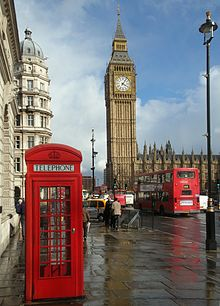
\includegraphics[width=0.3\linewidth]{london5.jpg}
\hspace{1 cm}
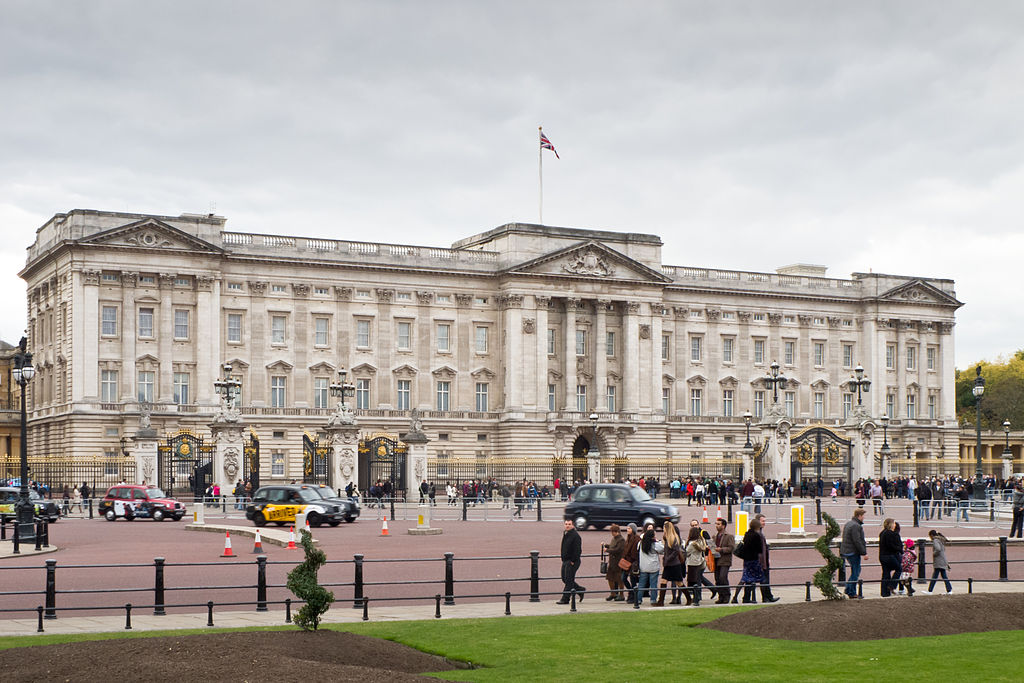
\includegraphics[width=0.5\linewidth]{london01.jpg}
\end{frame}

\begin{frame}
\frametitle{Немного древности}
Исторический центр города, образованный районами Вестминстер и Сити, 
сложился в викторианскую эпоху. 
Среди немногих построек, уцелевших здесь после пожара 1666 года, --- средневековая цитадель Тауэр.
\vskip 5 mm
\centering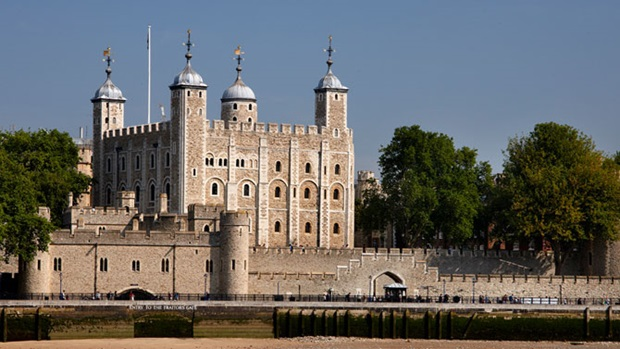
\includegraphics[width=0.6\linewidth]{london6.jpg}
\end{frame}

\begin{frame}
\frametitle{Немного о театрах}
Несколько крупных коммерческих театров, специализирующихся 
на постановке мюзиклов, 
комедий и драм, находятся в районе Вест-Энд. 
Существует даже специальный термин вест-эндский театр, 
использующийся в Англии для обозначения 
развлекательных коммерческих театров бродвейского типа. Из классических театров следует 
отметить Королевский национальный театр в районе Саут-Бэнк, новый театр «Глобус» и Театр при королевском дворе. 
\vskip 5 mm
\centering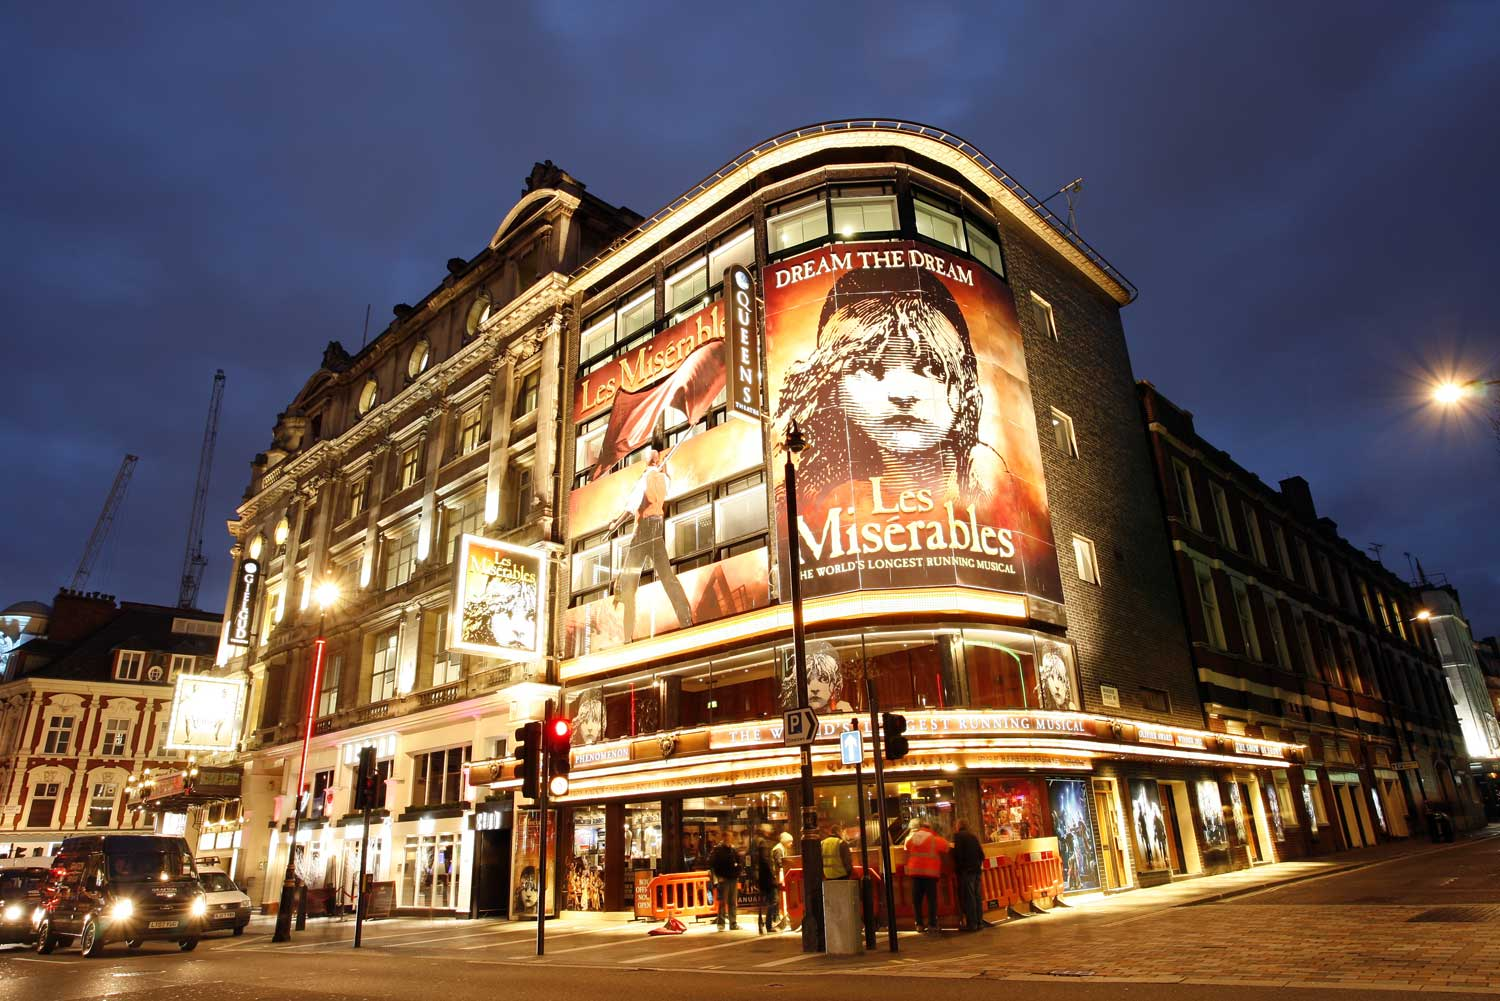
\includegraphics[width=0.4\linewidth]{london7.jpg}
\end{frame}

\begin{frame}
\frametitle{Хотел сделать о Москве, но до этого был урок английского}
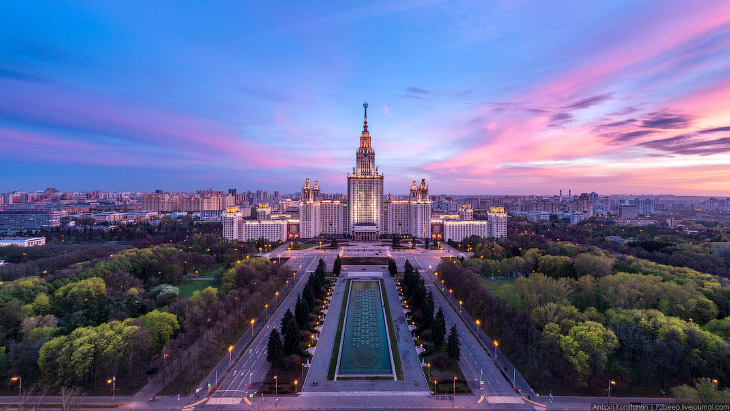
\includegraphics[width=0.5\linewidth]{moscow01.jpg}
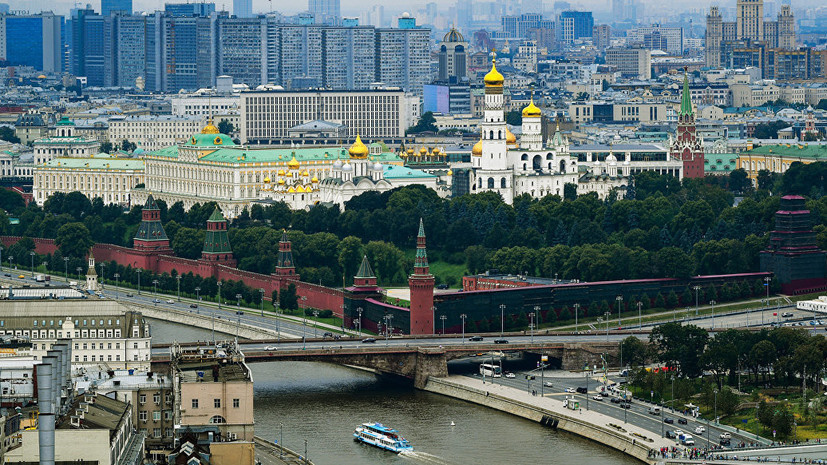
\includegraphics[width=0.5\linewidth]{moscow02.jpg}\\
\vskip 3 mm
\centering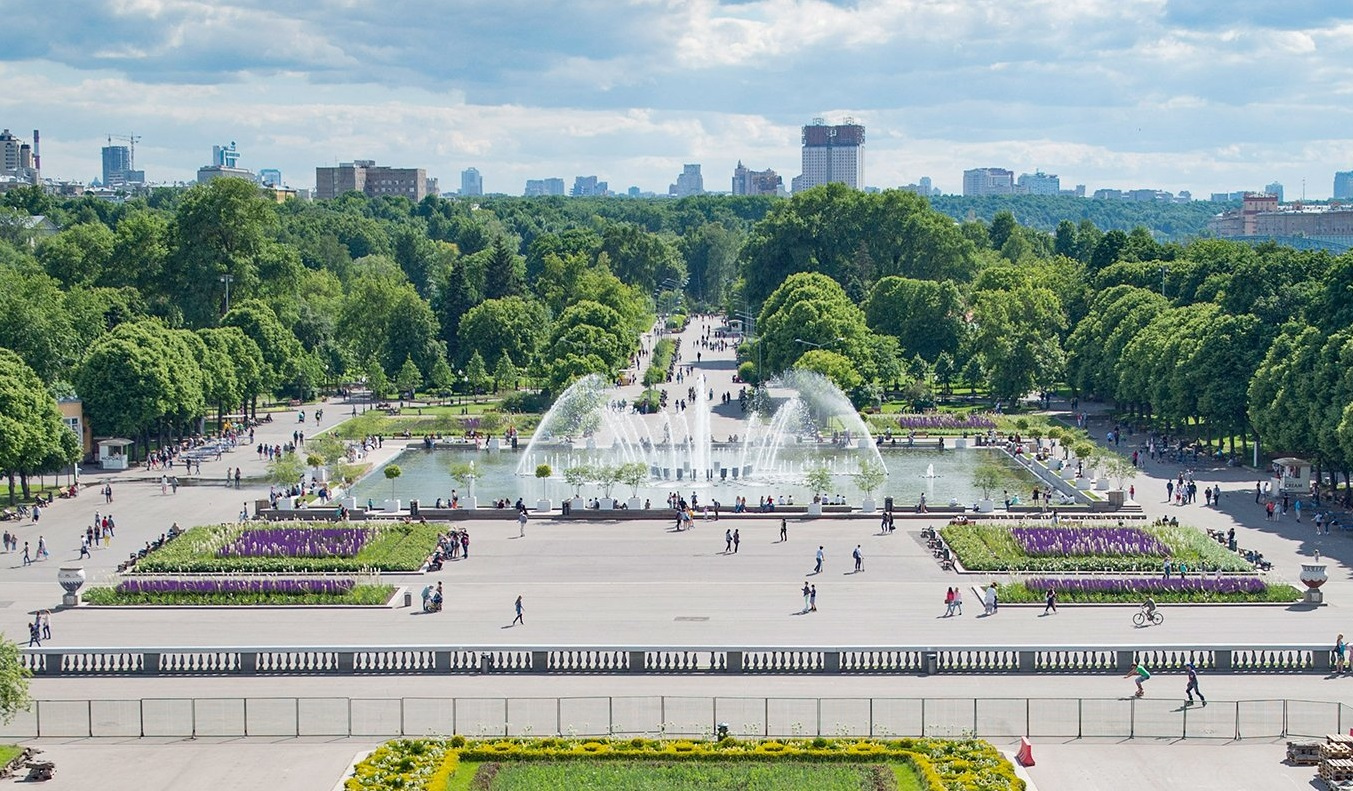
\includegraphics[width=0.6\linewidth]{moscow04.jpg}
\end{frame}

\begin{frame}
	\begin{center}
		{\large {\bf СПАСИБО ЗА ВНИМАНИЕ!}  }
	\end{center}
\end{frame}
\end{document}
